\section{Planning to Practice}
%%SL.2.24: It would be good to use a more inspiring section name (e.g., name it after the method or something like that). You might also consider separating the technical section into a general section about the conceptual method, and then a separate section with implementation details to explain how the method is instantiated
%%KF.3.1: Fixed

% Our aim is to study how we could enable a robot to efficiently learn to solve novel tasks by utilizing prior data of related tasks. 
% through compositionality. In this section, we outline an approach that facilitate online fine-tuning by planning with generated subgoals. 

% We propose Planning to Practice (PTP), an approach that efficiently fine-tunes a goal-conditioned policy to solve novel tasks.  
% by exploiting the compositional structure of the demonstration data.
%%SL.2.24: I think we need to be very clear about whether it's a method for learning from demonstrations, vs an RL method. Right now, the motivation mostly presents the method as an RL method, but we start throwing "demonstration" around, then people are likely to think it's an imitation learning method. We probably want to be clear on this point and avoid muddying the waters.
% In this section, we describe how online fine-tuning can be facilitated by using subgoals and provide a recipe for effectively searching for feasible plans by composing generated subgoals in the latent space.

% ----------------------------------------------------------------------------------------
% \subsection{Online Fine-Tuning by Composing Goals}

% Utilizing prior data: offline pre-training + online fine-tuning.
    % - Our goal: Fast adaptation to novel tasks
    % - Prior data
    % - How prior data can help
    % - Why prior data is not enough: Distribution shift + unseen combination of skills
    % - Offline pre-training using IQL
    % - Online fine-tuning 
% Our approach learns a goal-conditioned policy $\pi_{\theta}(a | s, s_g)$ for solving the target task specified by a desired final goal $s_g$. The goal-conditioned policy is pre-trained on a pre-collected offline dataset $\mathcal{D}_\text{offline}$ and then fine-tuned to reach $g$ by continuously collecting online data in the replay buffer $\mathcal{D}_\text{online}$. We expect $\mathcal{D}_\text{offline}$ to contain expert demonstrations of controlling the robot to perform diverse short-horizon interactions with the objects in the environment. \kuan{Add.}
% Through pre-training on such prior data, the policy $\pi$ could learn primitive behaviors that are potentially useful for solving the target tasks. Directly fine-tuning the policy to solve the target tasks can often lead to poor performance in the target task due to three major challenges. First, we do not assume to have access to unlimited amount of prior data and the under-trained policy often struggles to make any progress. Second, the policy needs to adapt to the distributional shift~\cite{} when the environment is initialized with object arrangements or lighting conditions unseen in the prior data. Third, we would like to robot to adapt to target tasks involving more complicated multi-stage interactions with the environment, thus the robot needs to learn novel strategies to compose the primitive behaviors across a longer time horizon.

%%SL.2.24: This is a bit abrupt right now, with lots of technical concepts provided without initial context for how they constitute a complete system. What I would suggest is to expand Section III to provide a problem statement, and then at the top of Section IV provide a high-level overview (perhaps with a diagram) that explains what are the constituent parts of the full system. Ideally these two things would introduce many of the symbols, such that when these symbols are used in this subsection, it won't be for the first time.
% Propose subgoals to facilitate online fine-tuning.
    % - Using subgoals to guide the fine-tuning.
    % - Switch subgoals.
    % - Summarize why this can help
We propose Planning to Practice (PTP), an approach that efficiently fine-tunes a goal-conditioned policy to solve novel tasks.  
To enable the robot to efficiently learn to solve the target task, we propose to use subgoals to facilitate the online fine-tuning of the goal-conditioned policy. Given the initial state $s_0$ and the goal state $s_g$, we search for a sequence of $K$ subgoals $\hat{s}_1:K = \hat{s}_1, ..., \hat{s}_K$ to guide the robot to reach $s_g$. Such subgoals will inform the goal-conditioned policy $\pi(a | s, s_g)$ what is the immediate next step on the path to $s_g$ and provide the policy more dense reward signals compared to directly using the final goal. We choose the sequence of subgoals at the beginning of each episode and feed the first subgoal in the sequence to the goal-conditioned policy. The policy will switch to the next subgoal in the sequence when the current subgoal is reached or the time budget assigned for the current subgoal runs out.

The main challenge is to search for a sequence of subgoals that can lead to the desired final goals while ensuring each subgoal is a valid state that can be reached from the previous subgoal. Particularly when the states correspond to full images, most vectors will not actually represent valid states, and indeed na\"{i}vely optimizing over image pixels may simply result in out-of-distribution inputs that lead to erroneous results when input into the goal-conditioned policy.
%The space of possible subgoal sequences is $|\mathcal{S}|^ K$ dimensional, which will make it computationally intractable to find the suitable subgoals for high-dimensional state spaces and long time horizons.

% Sampling-based planning
    % Overview
    % Sample trajectories using the affordance model
    % Choose the plan that corresponds to the lowest cost.
    % Considerations and challenges.
% Given the initial state $s_0$ and the goal state $s_g$, we use a planner to search for the sequence of subgoals through sampling-based planning. The planner aims to find the optimal sequence of subgoals $\hat{s}_{1:K}^*$ using the cost function $c(s_0, \hat{s}_{1:K}, s_g)$. To find the plan, we first sample $N$ sequences of subgoals $\hat{s}_{1:K}^1, ..., \hat{s}_{1:K}^N$ from the state space and evaluate the cost for each sequence. The sequence that corresponds to the lowest cost will be chosen as $\hat{s}_{1:K}^*$ for the goal-conditioned policy. 

%%SL.2.24: I would not refer to this as a planner habitually, because it doesn't really have the structure most would associate with a planning algorithm. I think it's OK (if you *really* want to) to call it a planner *after* explaining what it is, and then saying that it's a kind of planner. But definitely don't start calling it a planner out of the gate before explaining how it works, because it is very atypical for a planning method to work like this.
%%KF.3.1: Re-organized the paragraph as below.

As outlined in Fig.~\ref{fig:intro}, we devise a method to effectively propose and select valid subgoal sequences to guide online fine-tuning by means of a generative model. At the heart of our approach is a conditional subgoal generator $g(\cdot | s_0)$ that recursively produces candidate subgoals in a hierarchical manner conditioned on the initial state $s_0$. To find the optimal sequence of subgoals $\hat{s}_{1:K}^*$, we first sample $N$ candidate sequences $\hat{s}_{1:K}^1, ..., \hat{s}_{1:K}^N$ from the state space using the conditional subgoal generator. Then we rank the candidate sequences using a cost function $c(s_0, \hat{s}_{1:K}, s_g)$. The sequence that corresponds to the lowest cost will be selected as $\hat{s}_{1:K}^*$ for the goal-conditioned policy. Through this sampling-based planning procedure, we choose the subgoal for guiding the goal-conditioned policy $\pi$ during online fine-tuning. The overall algorithm is summarized in Algorithm~\ref{algo:ptp}. Next we describe the design of each module in details.

% Both the goal-conditioned policy and the conditional subgoal generator are pre-trained on the offline data. During the online fine-tuning, we use the planner to produce subgoals for the goal-conditioned policy.

% \kuan{Fix this.}.
% Both the goal-conditioned policy and the planner
% %%SL.2.24: goal-conditioned planner and planner? is there a typo here?
% %%AVN.2.26 fixed
% are pre-trained on the prior data. During the online fine-tuning, we use the planner to produce subgoals for the goal-conditioned policy. Through hindsight experience replay~\cite{}, the goal-conditioned policy is trained to reach not only the provided subgoals but also goals that it could achieve in the later stage of the episode. Eventually, the policy is supposed to learn to efficiently reach to distant goals even when the provided plans are sub-optimal. We evaluate the trained policy by directly feeding in the final goal in each target task.
%%SL.2.24: Organizationally, I wonder if it might be a good idea to have separate subsections to discuss the planner vs online finetuning. Perhaps logically, the better way to do it is to have an overview at the top, then explain latent space goal reaching, then talk about how its hard and explain affordances and planning, and then finetuning? Otherwise the explanation of planning prior to explaining affordances, latent spaces, or anything else is a bit hard to understand, and also doesn't actually fully explain our method, since many important details (e.g., the latent space and affordances) are omitted here and then "retrofitted" into the approach in later subsections.

% ----------------------------------------------------------------------------------------
\begin{algorithm}[t]
\caption{Planning To Practice (PTP)}
\begin{algorithmic}[1]
\Require set of final goals $\mathcal{G}$, time horizon $T$, offline data $\mathcal{D}_\text{offline}$, number of subgoals $K$.

\State Train $\pi(a | s, s_g)$ and $g(s, z)$ on $\mathcal{D}_\text{offline}$.
\State Initialize the online replay buffer $\mathcal{D}_\text{online} \leftarrow \varnothing$.

\While{not converged}
    \State Reset the environment and observe $s_0$.
    \State Sample $s_g$ from $\mathcal{G}$.
    \State Plan for the subgoals $\hat{s}_{1:K}$.
    
    \State $k \leftarrow 1$
    \For{$t = 1, ..., T$}
        \State Compute the action $a_t \leftarrow \pi(a_t | s_t, \hat{s}_K)$
        \State Observe the state $s_{t+1}$ and the reward $r_t$
        \State $\mathcal{D}_\text{online} \leftarrow \mathcal{D}_\text{online} \cup (s_t, a_t, r_t, s_{t+1})$.
        
        \If{$t \pmod {\Delta t} == 0$ \textbf{or} $|| s_{t+1} - \hat{s}_K || < \epsilon$}
            \State $k \leftarrow \min(k + 1, K)$ 
        \EndIf
    \EndFor
    
    \State Train $\pi$ on batches sampled from $\mathcal{D}_\text{offline}$ and $\mathcal{D}_\text{online}$.
    
\EndWhile

\end{algorithmic}
\label{algo:ptp}
% \vspace{-5mm}
\end{algorithm}


% ----------------------------------------------------------------------------------------
\subsection{Conditional Subgoal Generation}

% Use generative model to propose reachable goals.
    % Motivation: A way to efficiently generate diverse, high-fidelity, feasible sequences of subgoals for sampling-based planning. 
    % - What the affordance model is used for
    % - Recursive generation of subgoals
    % - A sequence of latent codes can be converted to a sequence of subgoals
    % - Propose goals at multiple timescales
    
%%SL.2.24: As written, it's not entirely clear what problem is being addressed -- it would be better if we can start the section by posing a question or stating the problem that actually requires this machinery.

The effectiveness of our planner relies on the generation of diverse and feasible sequences of subgoals as candidates. Specifically, we would like to generate the candidates by sampling from the distribution of suitable subgoal sequences $p(\hat{s}_1, ..., \hat{s}_K | s_0)$ conditioned on the initial state $s_0$. Most existing methods
%%SL.2.24: Not really clear which methods this is referring to.
%%KF.3.1: Fixed.
independently sample the subgoal at each step from a learned prior distribution~\citep{Pertsch2020LongHorizonVP} or a replay buffer~\citep{Eysenbach2019SearchOT}, which is unlikely to propose useful plans for tasks with large, combinatorial state spaces (i.e., with multiple objects).

We propose to break down $p(\hat{s}_1, ..., \hat{s}_K | s_0)$ into $p(\hat{s}_1 | s_0) \Pi_{i=1}^k p(\hat{s}_i | \hat{s}_{i - 1})$ through modeling the conditional distribution $p(s' | s)$ of the reachable next subgoal $s'$. By utilizing temporal compositionality, the conditional subgoal generation paradigm improves generalization and enables generation of sequences of arbitrary lengths.
%%KF.3.1: The last sentence might be hard to follow. Fix this if have time.

We use a conditional variational encoder (CVAE)~\citep{sohn2015cvae} to capture the distribution of reachable goals $p(s' | s)$. In the CVAE, we define the decoder as $g(s, z)$ and the encoder as $q(z | s, s')$, where $z$ is the learned latent representation of the transitions and it is sampled from a prior probability $p(z)$. To propose a sequence of subgoals, we use $g(s, z)$ as the conditional subgoal generator. Conditioned on the initial state $s_0$, the first subgoal $\hat{s}_1$ can be generated as $\hat{s}_1 = g(s_0, z_1)$ given the sampled $z_1$. Then the $i_\text{th}$ subgoal can be recursively generated by sampling $z_i \sim p(z)$ and computing $\hat{s}_i = g(\hat{s}_{i - 1}, z_i)$ given the previous subgoal $\hat{s}_{i - 1}$. In this way, we could sample a sequence of i.i.d. latent representations $z_1, ..., z_K$ and recursively generate $\hat{s}_1, ..., \hat{s}_K$ conditioned on the initial state $s_0$ using the conditional subgoal generator.

% Training of the affordance model
    % - Trained for what
    % - Sample sequences for training
    % - Training with recursive generation. No backpropagation through time
    % - Handle compounding errors: Randomly choose between the gt context and the previously generated context.
    % - Training at different time scales
The CVAE is trained to minimize the evidence lower bound (ELBO)~\citep{kingma2014vae} of $p(s' | s)$ given the offline dataset $\mathcal{D}$. During training, we sample transitions $(s_t, s_{\tau})$ from the offline dataset to form the minibatches, where $\tau = t + \Delta t$ is a future step that is $\Delta t$ steps ahead. Instead of using a fixed $\Delta t$, we sample $\Delta t$ from a range for each transition to provide richer data. To encourage the trained model to be robust to compounding errors, we sample sequences composed of multiple states and use the subgoal reconstructed at the previous step as the context in the next step. Therefore, the objective for training the conditional subgoal generator is:
\begin{equation}
    \mathbb{E}_{q(z | s_t, s_{\tau})}||s_{\tau} - g(s_t, z)||^2 + \ensuremath{D_{KL}[q(z | s_t, s_{\tau}) || p(z)]}
    \label{eqn:elbo}
\end{equation}
where $\ensuremath{D_{KL}[\cdot || \cdot]}$ indicates the KL-Divergence.

% We train the conditional goal generator at different time scales.  

% Architecture of the affordance model
    % - Considerations: High efficiency & low compounding errors & diversity % samplable
    % - CCVAE
    % - UNet architecture 
    % - Discretization reduces the compounding errors 
% Latent state using VQVAE
    % - Use VQVAE encoding to generate states of high-dimensional.
    % - Pretraining VQVAE.
    % - Why this is not enough.
    % - Challenges. (static v.s. dynamic properties)
% To enhance the quality of the generated states, we use a U-Net architecture in the CVAE to preserve the information of different spatial granularities and perform vector quantization at the output layer. It is hard to conduct planning and checking if a goal is reached in the pixel space. Following the practice of \cite{}, we use a extract latent representations of the states using a Vector Quantized Variational Autoencoder (VQ-VAE)~\cite{}. For simplicity, we directly use $s$ to denote the VQ-VAE representations of the states in the rest of the paper. The VQ-VAE is pretrained on the prior data and its weights are fixed in the rest of the training process. 
% This paragraph should probably be moved to the Experiments section as an implementation detail.

% ----------------------------------------------------------------------------------------
\subsection{Efficient Planning in the Latent Space}

% ----------------------------------------------------------------------------------------
\begin{algorithm}[t]
\caption{$Plan(s_0, s_g, L, K, M, N)$}
\begin{algorithmic}[1]
\Require the initial state $s_0$, the goal state $s_g$, number of subgoals $K$, number of levels $L$, multiplier $M$, number of samples $N$.

\State Sample $N$ latent action sequences $\{z_{1:K}^i\}_{i=1}^N$.
\State Recursively generate subgoals $\{\hat{s}_{1:K}^i\}_{i=1}^N$ using $g(s, z)$.
\State Select $z_{1:K}^*$ and $\hat{s}_{1:K}^*$ of the lowest cost.
\State Update $z_{1:K}^*$ and $\hat{s}_{1:K}^*$ using MPPI.

\If{L = 1}
    \State \Return $\hat{s}_{1:K}^*$
\Else
    \State Denote $\hat{s}_0^* \leftarrow s_0$.
    \State Initialize the plan $\hat{\mathcal{S}}$ as an empty list
    \For{$i = 1, ..., K$}
        \State Append $Plan(\hat{s}_{i-1}^*, \hat{s}_{i}^*, L - 1, M, M, N)$ to $\mathcal{S}$
    \EndFor
    \State \Return $\hat{\mathcal{S}}$
\EndIf

\end{algorithmic}
\label{algo:planning}
\end{algorithm}
% \vspace{-5mm}

% To tackle the large variety of possible subgoal sequences, we build a planner that efficiently searches for sequences of subgoals in the latent space as shown in Algorithm~\ref{algo:planning}. Built upon the Model Predictive Path Integral (MPPI)~\cite{Gandhi2021RobustMP}, the planner  performs importance sampling by iteratively optimizing and perturbing the plan in the learned latent space of the conditional subgoal generator. The learned latent space captures the diverse interactions that the robot can perform given a state. A small perturbation in the latent space might result in very different generated subgoals. To address these issues, we propose two techniques to enable the planner to robustly search for the optimal plan in such a high-dimensional space.

%%SL.2.24: Generally, this paragraph is pretty hard to follow, and is a bit too vague to be well understood.

We build a planner that efficiently searches for sequences of subgoals in the latent space as shown in Algorithm~\ref{algo:planning}. To tackle the large search space of candidate subgoal sequences, we design a hierarchical planning algorithm that searches for subgoals in a coarse-to-fine manner and re-use the previously selected subgoals as candidates in new episodes.

% Hierarchical planning.
    % - Divide and conquer
    % - From coarse to fine
    % - Fixed resolution
    % - Similar to GCP, but conditional generation enables temporal extension and better generalization
    % - 
% We design a hierarchical planning algorithm with the conditional subgoal generator to reduce the search space. 
% Instead of generating the subgoals sequentially and evaluate the cost of the whole sequence holistically, we propose to generate and search for the subgoals in a coarse-to-fine manner. 
The hierarchical planning is conducted at $L$ levels with different temporal resolutions $\Delta t_1$, ..., $\Delta t_L$. The temporal resolution of each level is an integral multiple of that of the previous level, \ie, $\Delta t_i = M \Delta t_{i - 1}$, where $M$ is a scaling factor and is set to 2 in our experiments. We first plan for the subgoals $\hat{s}_1^1, \hat{s}_2^1, ...$ on the first level. Then the subgoals $\hat{s}_{1:K}^l$ of finer temporal resolution are planned on each level $l$ to connect the subgoals planned on the previous level $l-1$. Specifically, given the adjacent subgoals $\hat{s}_i^{l-1}$ and $\hat{s}_{i+1}^{l-1}$ produced on the previous level, we plan for a segment of  $M$ subgoals $\hat{s}_{i * M + 1}^{l}, ..., \hat{s}_{(i+1) * M}^{l}$ on the level $l$, by treating $\hat{s}_i^{l-1}$ and $\hat{s}_{i+1}^{l-1}$ as the initial state and final goal state in Eqn.~\ref{eqn:cost_function}. The planned segments are returned to the previous level and concatenated as a more fine-grained plan. For this purpose, we train $L$ conditional subgoal generators to propose subgoals that are $\Delta t_1$, ..., $\Delta t_L$ steps away, respectively. In contrast to the prior work~\citep{Pertsch2020LongHorizonVP}, the conditional subgoal generators enable us to plan for unseen goals that are beyond the temporal horizon of the demonstrations in the offline dataset by exploiting the compositional structure of the demonstrations. By recursively generating the subgoals across time at each level, we only need to enforce that the temporal resolution of the top level $\Delta t_L$ is smaller than since the the conditional subgoal generator $f^{1}(s, z)$ needs to be trained on trajectories at least $\Delta t_L + 1$ steps in length. 

% Latent plan buffer.
    % - Sensitive to the initialization
    % - In practice, we find that..., if we sample from the prior
    % - We keep a buffer
    % - Every episode, store
    % - Sample from both the prior and the buffer
We maintain a latent plan buffer for each level to further facilitate the planning with the conditional subgoal generator. After each episode, the selected latent representations on each level are appended to the corresponding latent plan buffer. In each target task, the subgoals are supposed to have the same semantic meaning. In spite of the variations of the initial and goals state in each episode, the optimal plans in the latent space can often be similar to each other. Therefore, we sample half of the latent representations from the prior distribution $p(z)$ and the other half from the latent plan buffer among the initial samples to enhance the chance of finding a close initial guess. 

We build our planner upon the model predictive path integral (MPPI)~\citep{Gandhi2021RobustMP}, which iteratively optimizes the plan through importance sampling. In each interaction, we perturb the chosen plan in the latent space with a small Gaussian noise as new candidates. 

\begin{figure}[ht!]
    \centering
    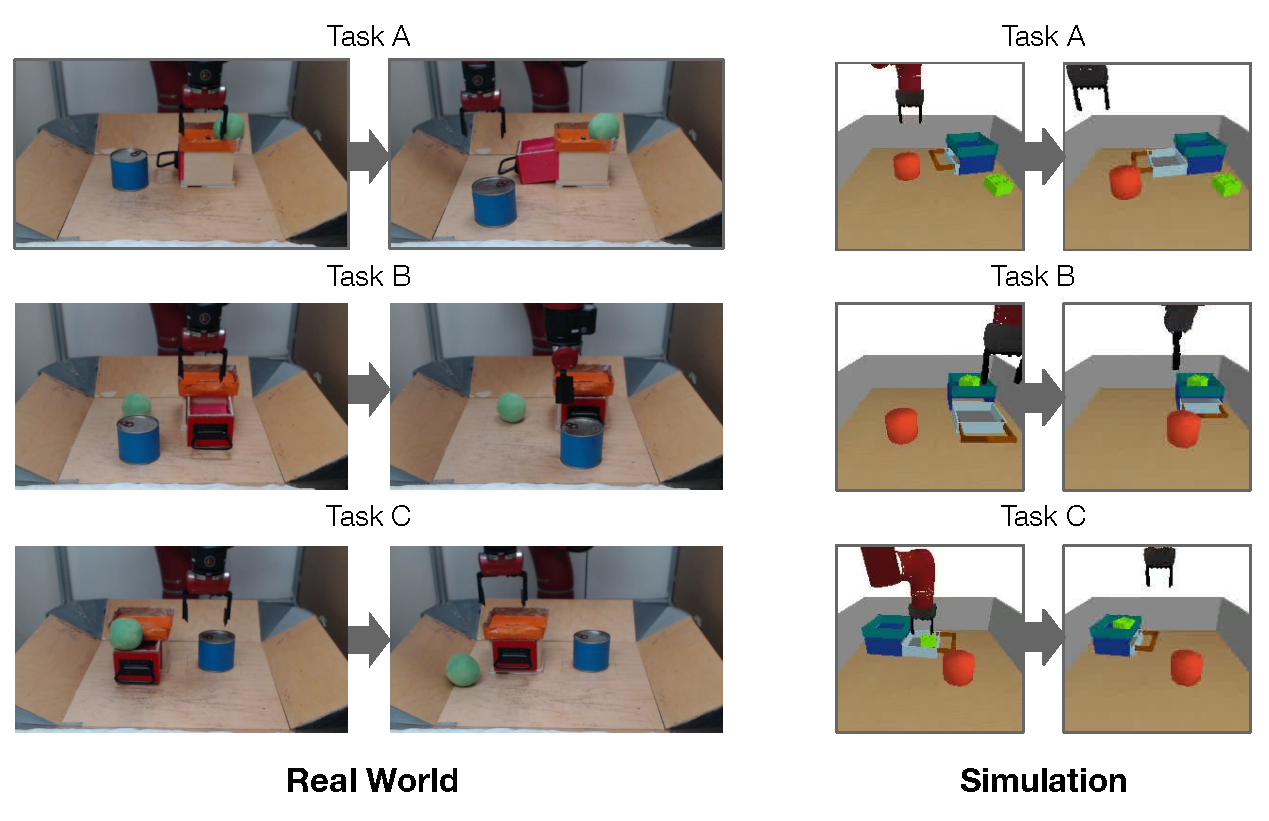
\includegraphics[width=.8\textwidth]{ptp/figures/target_tasks.pdf}
    \vspace{-3mm}
    \caption{\textbf{Target tasks.} Three multi-stage tasks are designed for our experiments in the simulation and the real world respectively. In each target task, the robot needs to strategically interacts with the environment (\eg first takes out an object in the drawer then closes the drawer). The initial state and the desired goal state are shown for each task. }
    %\vspace{-5mm}
    \label{fig:target_tasks}
\end{figure}

\vspace*{.3cm}
\begin{figure*}[ht!]
    \centering
    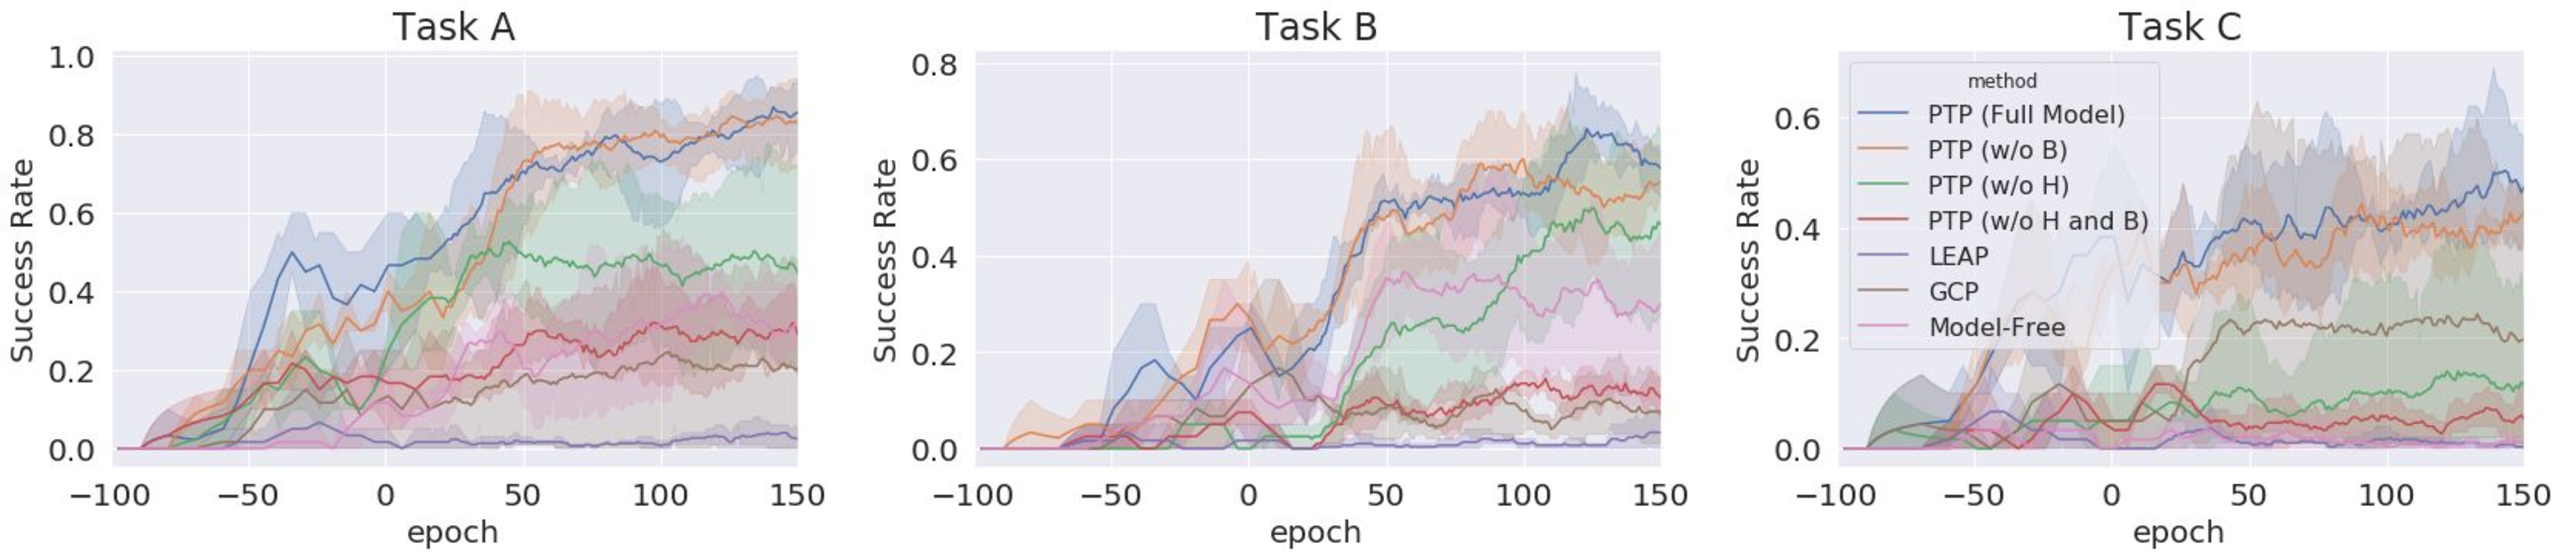
\includegraphics[width=0.95\textwidth]{ptp/figures/sim_quantitative.pdf}
    \vspace{-3mm}
    \caption{
    \textbf{Quantitative comparison in simulation.} The average success rate across 3 runs is shown with the shaded region indicating the standard deviation. The negative x-axis indicates the epochs of offline pre-training and positive x-axis indicates epochs of online fine-tuning.  
    % This figure will show the success rates of all methods (including the baselines and ablations) for the three target tasks.
    Using offline learning and planning, our method PTP is able to solve these tasks partially (at 0 epochs).
    Then with online finetuning the performance improves further.
    In contrast, prior methods have lower offline performance and do not fine-tune successfully in most cases, as they do not collect coherent online data.
    }
    %\vspace{-5mm}
    \label{fig:sim_quantitative}
\end{figure*}

% ----------------------------------------------------------------------------------------
\subsection{Cost Function For Feasible Subgoals}

% Planing objective. 
    % - Intuition: Reach the goal & transitions should be probable
    % - Reach the goal
    % - Sampling from the affordance model encourages the transitions to be likely.
% At beginning of each episode, we plan for a sequence of feasible subgoals that leads to the desired goal state of the target task from the initial state. The subgoals are chosen through sampling-based planning, in which we first sample $n$ sequences of subgoals $\hat{s}_{0:k}$ using the conditional goal generator and then evaluate the cost $c(\hat{s}_{0:k})$ of each sequence. 

To provide informative guidance to the policy $\pi(a | s, s_g)$, we would like that the final goal $s_g$ can be reached at the end of the episode while encouraging the transition between each pair of subgoals to be feasible within a limited time budget. As explained in Sec.~\ref{sec:preliminaries}, the goal state is considered to be reached when the Euclidean distance
%%SL.2.24: The Euclidean distance bit will come across as pretty confusing, given that previously we talked about using images -- so readers will wonder, does this mean that we are doing Euclidean distance over images? But that doesn't really make sense.
%%KF.3.1: Clarified.
between the last subgoal in the plan and the desired goal is less than a threshold $\delta$ in the learned latent space. The feasibility of each transition between adjacent subgoals can be measured using the goal-conditioned value function $V(s, s')$ trained by the reinforcement learning algorithm. Therefore, finding the subgoals $\hat{s}_{1:K}^*$ can be formulated as a constrained optimization problem: 
\begin{eqnarray}\label{eqn:constrained_optimization}
    \text{minimize} 
    & \quad & ||s_g - \hat{s}_K|| \\
    \text{subject to} 
    % & \quad & V(s_0, \hat{s}_1) \geq \delta\\
    & \quad & V(\hat{s}_i, \hat{s}_{i+1}) \geq \delta, \text{for $i = 0, ..., K-1$} \nonumber
\end{eqnarray}
where we use $\hat{s}_0 = s_0$ to denote the initial state for convenience. By re-writing Eq.~\ref{eqn:constrained_optimization} as a Lagrangian,
%%SL.2.24: The previous equation has three terms, but perhaps it can be written more concisely so that there is just one constraint (i.e., the line V(s_0, \hat{s}_1) \geq \delta is omitted), if we are careful with our notation.
%%KF.3.1: Fixed.
we obtain the cost function with a weight $\eta$:
\begin{equation}
    c(s_0, \hat{s}_{1:K}, s_g) = ||s_g - \hat{s}_K|| + \eta \sum_{i=0}^{K-1} V(\hat{s}_i, \hat{s}_{i+1})
    \label{eqn:cost_function}
\end{equation}
% where $\eta$ is a weight that balances the two terms. 
The details of our method are explained in Sec.~\ref{sec:implementation_details}.